\section{Datenbank--Schema}

\subsection{Konzeptuelles Datenbankschema: Entity--Relationship Diagram}

Hier werden die Gegenstände der realen Welt modelliert wie in Abbildung \ref{fig:erd} gezeigt modelliert. Hierbei ist zu beachten, dass die Entität „Frage“ das zentrale Element des Datenmodells darstellt. Die weiteren Entitäten „Antwortmöglichkeit“ bzw. „gegebene Antwort” sind existenzabhängige Entities. Ohne Antwortmöglichkeit kann ohne zugehörige Frage nicht existieren, eine gegebene Antwort macht nur Sinn, wenn es eine entsprechende Antwortmöglichkeit und Frage gibt.

Die Entität „Benutzer“ steht in keiner Beziehung zu den anderen Entitäten, sie wird auch nur für die Eingabe neuer Fragen und Antwortmöglichkeiten, bzw. zur Authentifizierung benötigt.

\begin{figure}[H]
\begin{center}
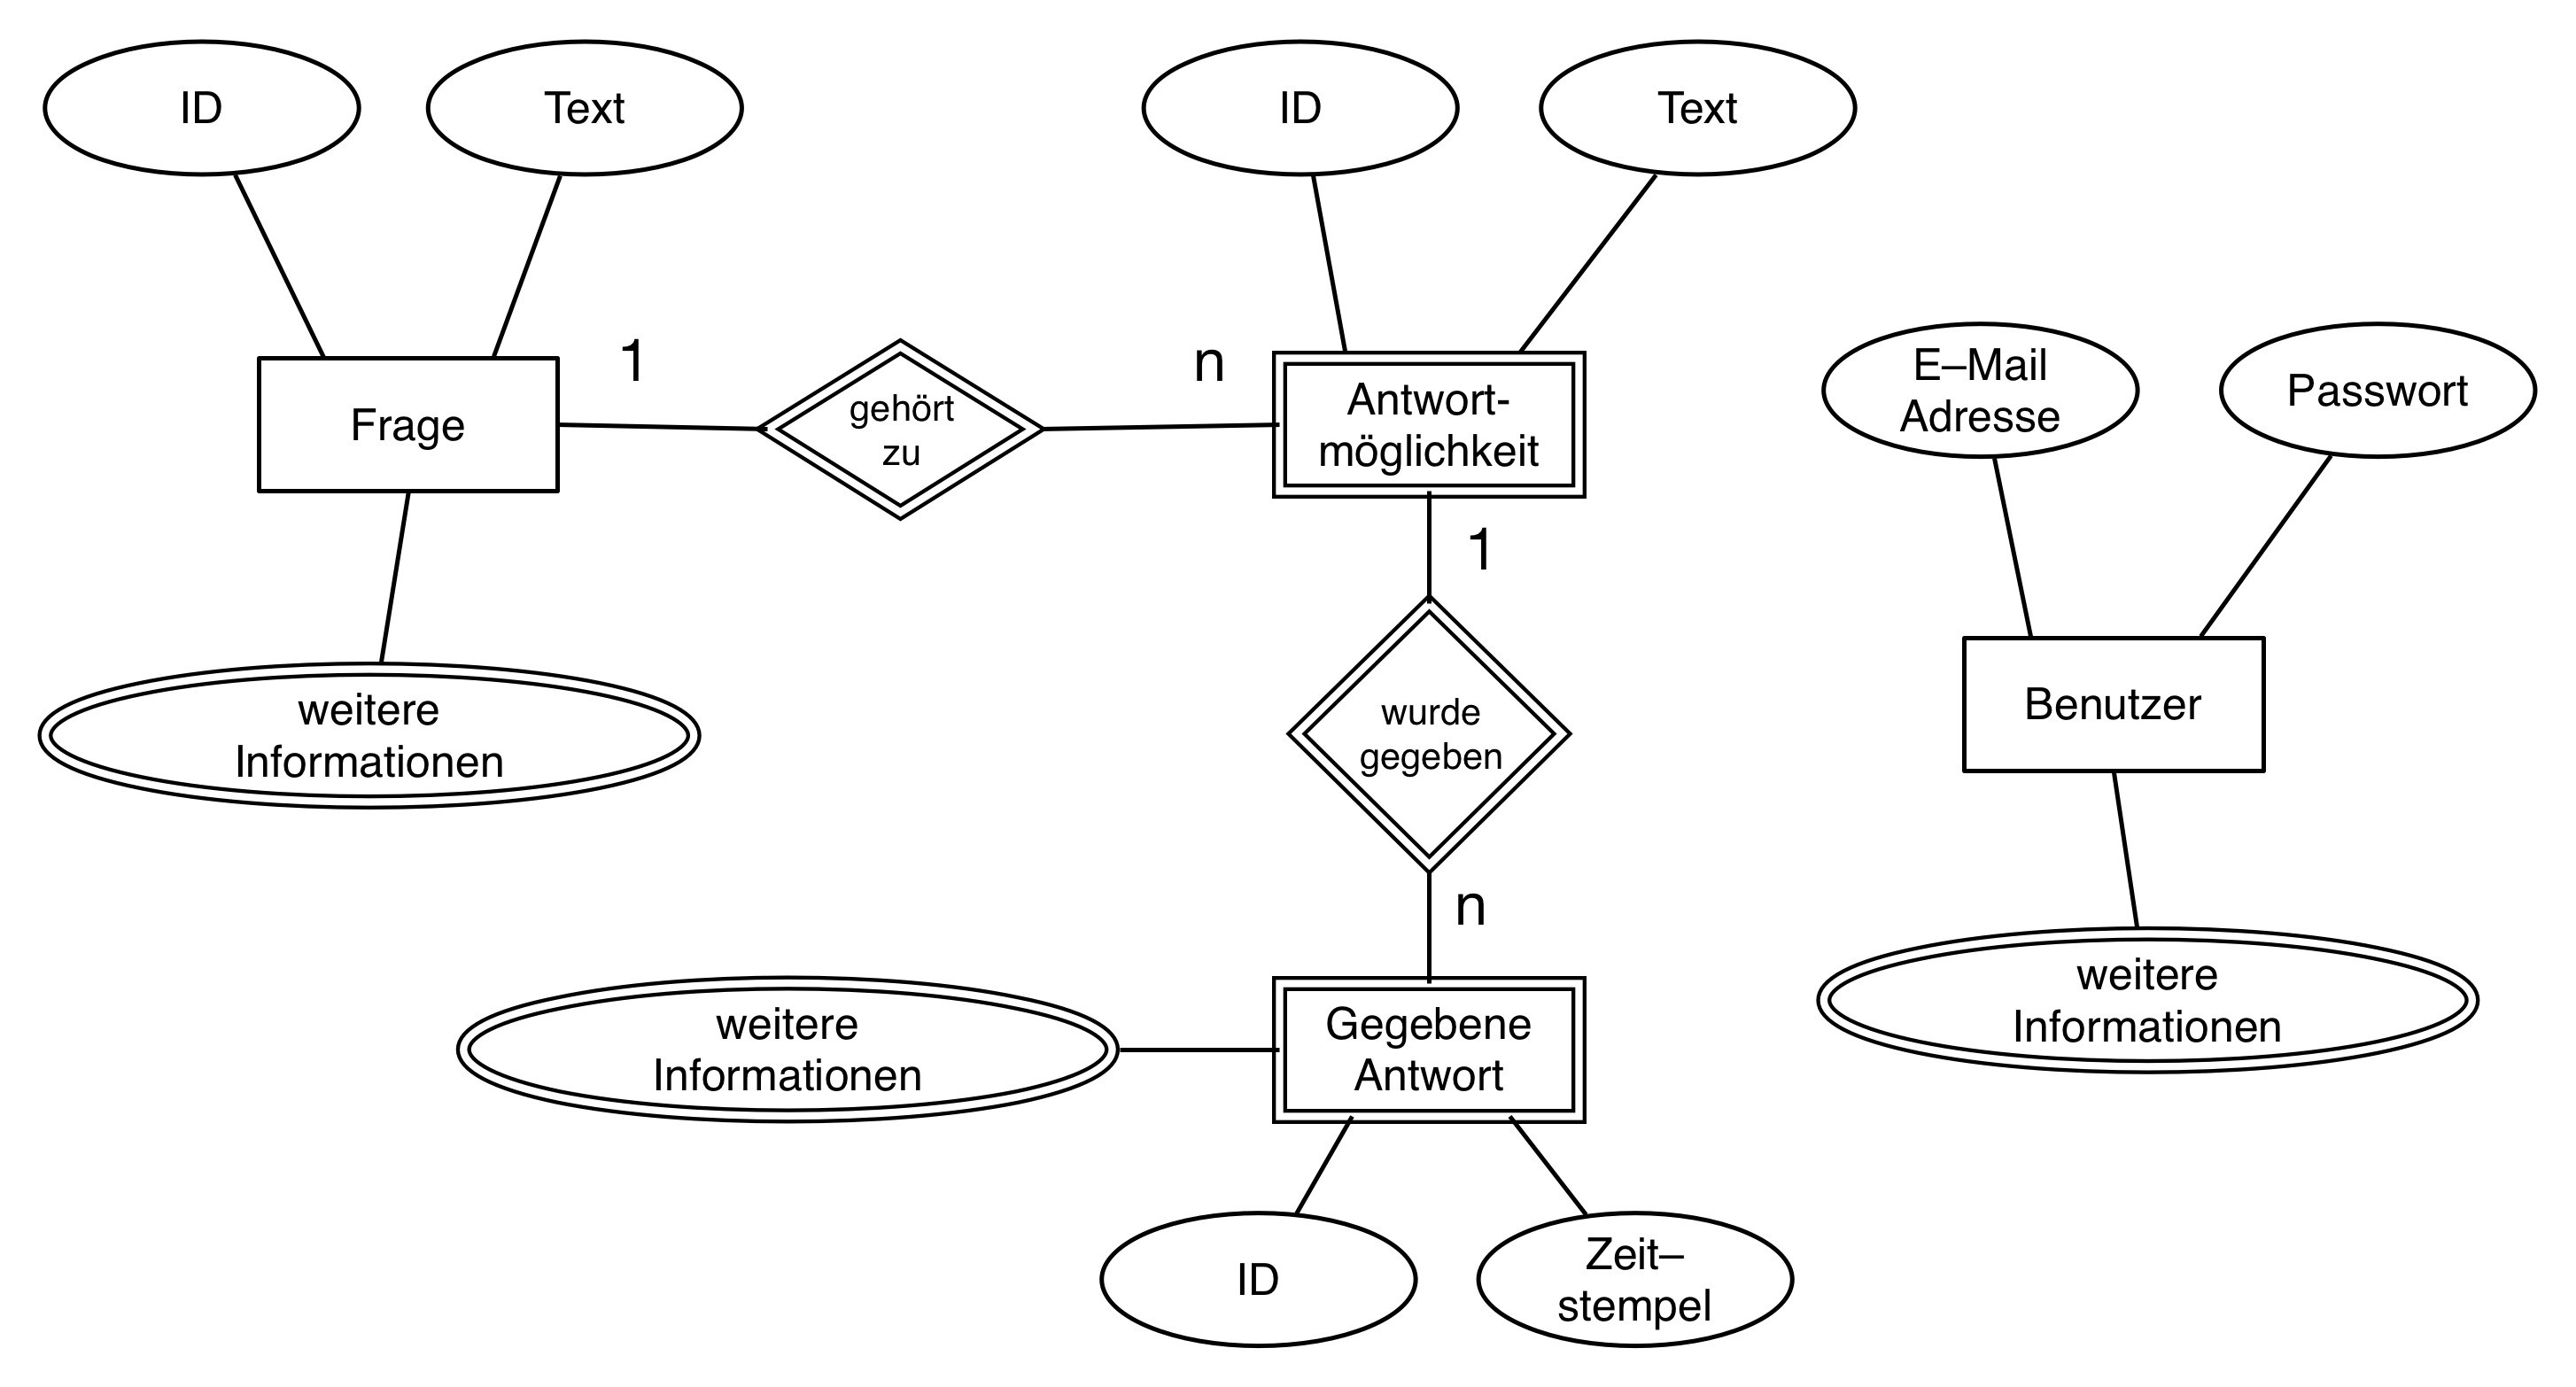
\includegraphics[width=\textwidth]{ERD.jpg}
\caption{Entity Relationship Diagram}
\end{center}
\label{fig:erd}
\end{figure}

Die als zsammengesetzte Attribute dargestellten „weiteren Informationen“ sind Attribute der jeweiligen Entitäten, die für die gestellten Anforderungen nicht notwendig sind, jedoch im Produktivbetrieb großen Zusatznutzen bieten könnten. So wäre es möglich die gegebenen Antworten durch die Speicherung der IP--Adresse, Browser--Fingerprinting\footnote{Die Identifikation eines speziellen Nutzers durch Konfigurationsdetails des Webbrowsers, Bildschirmgröße, Betriebssystemversion, etc. Siehe auch \url{https://panopticlick.eff.org/}} oder andere Techniken genauer zu identifizieren und somit einem bestimmten Nutzer zuzuordnen. Hierbei sind dann die jeweiligen Datenschutzbestimmungen zu beachten.

Die Datensätze der Entity „Frage“ könnten Zeitangaben enthalten, die festlegen wann bzw. wie lange eine Frage auf der Website angezeigt wird. Die Antwortmöglichkeiten könnten durch entsprechende Angaben zur Sortierreihenfolge geordnet werden.

\subsection{Logisches Datenbankschema: Entity--Relationship Diagram}

Aufgrund des in Abbildung \ref{fig:erd} auf Seite \pageref{fig:erd} dargestelten Modell ergibt sich folgende Relationen:


\subsection{Tabelle: user}
\begin{center}
\tablehead{ \textbf{user} & & 
\\ }
\bottomcaption[Beschreibung]{Beschreibung. Quelle: Berger, Vorlesung, 2012, München }
\begin{supertabular}{c|c|c}
\hline
email & varchar(255) &  \\
pw & char(32) &  \\
\end{supertabular}
\end{center}


\begin{figure}[h]
\begin{minted}[bgcolor=bg]{sql}
CREATE TABLE user (
  email VARCHAR(255) NOT NULL,
  pw CHAR(32) NOT NULL,
  create_time TIMESTAMP DEFAULT CURRENT_TIMESTAMP,
  PRIMARY KEY (`email`));
\end{minted}
\caption{SQL: CREATE TABLE user}
\label{sql:tbluser}
\end{figure}

Als Benutzername wird hierbei die E--Mail Adresse des Administrators genutzt. 

Das Passwort sollte nicht im Klartext in der Datenbank gespeichert werden. Ein \code{salted hash}\footnote{Also der Hashwert des Passworts, welches zuvor mit Applikationsspezifischen Zusatzdaten ergänzt wurde} schützt hier das Passwort vor dem Ausspähen durch den Administrator selbst\footnote{Seit Vodafone 2013 eine dokumentierte Gefahr} oder durch Angreifer.\\
Die hier reservierten 32 Byte sind für den in der MySQL--Dokumentation\footnote{\cite{mysql-pcrypt}} emphohlenen MD5-Hash ausreichend. Da die entsprechende PHP--Dokumentation\footnote{\cite{php-pcrypt}} hier allerdings eine genau entgegengesetzte Empfehlung gibt, ist dieser Sicherheitsaspekt für ein Produktivsystem nochmals genauer zu prüfen.

\subsection{Tabelle: frage}
\begin{figure}[h]
\begin{minted}[bgcolor=bg]{sql}
CREATE TABLE frage (
  fid INT NOT NULL AUTO_INCREMENT,
  txt VARCHAR(1024) NOT NULL,
  PRIMARY KEY (`fid`));
\end{minted}
\caption{SQL: CREATE TABLE frage}
\label{sql:tblfrage}
\end{figure}

\subsection{Tabelle: antwort}
\begin{figure}[h]
\begin{minted}[bgcolor=bg]{sql}
CREATE TABLE antwort (
  aid INT NOT NULL AUTO_INCREMENT,
  nr  INT NULL,
  txt VARCHAR(1024) NOT NULL,
  fid INT NOT NULL,
  PRIMARY KEY (`aid`),
  FOREIGN KEY (`fid`) REFERENCES frage(`fid`));
\end{minted}
\caption{SQL: CREATE TABLE antwort}
\label{sql:tblantwort}
\end{figure}

\subsection{Tabelle: geantwortet}
\begin{figure}[h]
\begin{minted}[bgcolor=bg]{sql}
CREATE TABLE geantwortet (
  gid INT NOT NULL AUTO_INCREMENT,
  aid INT NOT NULL,
  zs TIMESTAMP DEFAULT CURRENT_TIMESTAMP,
  PRIMARY KEY (`gid`),
  FOREIGN KEY (`aid`) REFERENCES antwort(`aid`));
\end{minted}
\caption{SQL: CREATE TABLE geantwortet}
\label{sql:tblgeantwortet}
\end{figure}

\subsection{Query: Frage -- Text}
Wird für die Abfrage und Auswertung benötigt.

\begin{figure}[h]
\begin{minted}[bgcolor=bg]{sql}
select txt from frage where fid = <n>;
\end{minted}
\caption{SQL: Text von Frage <n>}
\label{sql:qfragetxt}
\end{figure}

\subsection{Query: Antwortmöglichkeiten}
Wird für die Abfrage benötigt.

\begin{figure}[h]
\begin{minted}[bgcolor=bg]{sql}
select antwort.txt
	from antwort
	where fid = <n> 
\end{minted}
\caption{SQL: Mögliche Antworten für Frage <n>}
\label{sql:qantwnum}
\end{figure}


\subsection{Query: Anzahl der gegebenen Antworten}
Wird für die Auswertung benötigt: 100\%

\begin{figure}[h]
\begin{minted}[bgcolor=bg]{sql}
select count(geantwortet.aid) 
	from antwort, geantwortet 
	where geantwortet.aid = antwort.aid and antwort.fid = <n>;
\end{minted}
\caption{SQL: Antwortzahl 100\% von Frage <n>}
\label{sql:qantw100}
\end{figure}

\subsection{Query: Gegebene Antworten und Häufigkeit}
Wird für die Auswertung benötigt.

\begin{figure}[h]
\begin{minted}[bgcolor=bg]{sql}
select antwort.txt, count(geantwortet.aid) 
	from antwort, geantwortet 
	where geantwortet.aid = antwort.aid and antwort.fid = <n> 
	group by geantwortet.aid;
\end{minted}
\caption{SQL: Gegebene Antworten mit Häufigkeit für Frage <n>}
\label{sql:qantwnum}
\end{figure}




\subsection{Tabelle}

\begin{center}
\tablehead{ \textbf{Head1} & \textbf{Head2} & \textbf{Head3}
\\ }
\bottomcaption[Beschreibung]{Beschreibung. Quelle: Berger, Vorlesung, 2012, München }
\begin{supertabular}{c|c|c}
\hline
1 & 2 & 3 \\
4 & 5 & 6 \\
7 & 8 & 9 \\
1 & 2 & 3 \\
4 & 5 & 6 \\
7 & 8 & 9 \\
\end{supertabular}
\end{center}

\subsection{Bilder}

\begin{figure}[H]
\begin{center}
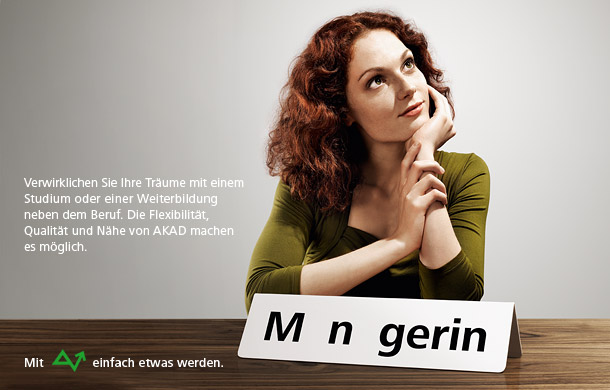
\includegraphics[scale=0.5]{akad_bild1.jpg}
\caption[Akad]{Akad. Quelle: www.akad.de}
\end{center}
\end{figure}

\subsection{Syntax Highlighting}
\begin{figure}[h]
\begin{minted}[bgcolor=bg]{php}
<?php 
$title="Lorem";
$desc = "Lorem Ipsum";
include($_SERVER['DOCUMENT_ROOT'].'/header.php'); 
?>
\end{minted}
\caption{Quellcode: Aufruf von header.php (PHP)}
\label{abb:header}
\end{figure}
